\documentclass[a4paper]{article}
\usepackage[spanish]{babel}
\usepackage[utf8]{inputenc}
\usepackage{charter}   % tipografia
\usepackage{graphicx}
%\usepackage{makeidx}
\usepackage{paralist} %itemize inline

%\usepackage{float}
%\usepackage{amsmath, amsthm, amssymb}
%\usepackage{amsfonts}
%\usepackage{sectsty}
%\usepackage{charter}
%\usepackage{wrapfig}
%\usepackage{listings}
%\lstset{language=C}


\usepackage{color} % para snipets de codigo coloreados
\usepackage{fancybox}  % para el sbox de los snipets de codigo

\definecolor{litegrey}{gray}{0.94}

% \newenvironment{sidebar}{%
% 	\begin{Sbox}\begin{minipage}{.85\textwidth}}%
% 	{\end{minipage}\end{Sbox}%
% 		\begin{center}\setlength{\fboxsep}{6pt}%
% 		\shadowbox{\TheSbox}\end{center}}
% \newenvironment{warning}{%
% 	\begin{Sbox}\begin{minipage}{.85\textwidth}\sffamily\lite\small\RaggedRight}%
% 	{\end{minipage}\end{Sbox}%
% 		\begin{center}\setlength{\fboxsep}{6pt}%
% 		\colorbox{litegrey}{\TheSbox}\end{center}}

\newenvironment{codesnippet}{%
	\begin{Sbox}\begin{minipage}{\textwidth}\sffamily\small}%
	{\end{minipage}\end{Sbox}%
		\begin{center}%
		\vspace{-0.4cm}\colorbox{litegrey}{\TheSbox}\end{center}\vspace{0.3cm}}



\usepackage{fancyhdr}
\pagestyle{fancy}

%\renewcommand{\chaptermark}[1]{\markboth{#1}{}}
\renewcommand{\sectionmark}[1]{\markright{\thesection\ - #1}}

\fancyhf{}

\fancyhead[LO]{Sección \rightmark} % \thesection\ 
\fancyfoot[LO]{\small{Nombre Apellido, Nombre Apellido, Nombre Apellido}}
\fancyfoot[RO]{\thepage}
\renewcommand{\headrulewidth}{0.5pt}
\renewcommand{\footrulewidth}{0.5pt}
\setlength{\hoffset}{-0.8in}
\setlength{\textwidth}{16cm}
%\setlength{\hoffset}{-1.1cm}
%\setlength{\textwidth}{16cm}
\setlength{\headsep}{0.5cm}
\setlength{\textheight}{25cm}
\setlength{\voffset}{-0.7in}
\setlength{\headwidth}{\textwidth}
\setlength{\headheight}{13.1pt}

\renewcommand{\baselinestretch}{1.1}  % line spacing


% \setcounter{secnumdepth}{2}
\usepackage{underscore}
\usepackage{caratula}
\usepackage{url}


% ******************************************************** %
%              TEMPLATE DE INFORME ORGA2 v0.1              %
% ******************************************************** %
% ******************************************************** %
%                                                          %
% ALGUNOS PAQUETES REQUERIDOS (EN UBUNTU):                 %
% ========================================
%                                                          %
% texlive-latex-base                                       %
% texlive-latex-recommended                                %
% texlive-fonts-recommended                                %
% texlive-latex-extra?                                     %
% texlive-lang-spanish (en ubuntu 13.10)                   %
% ******************************************************** %



\begin{document}


\thispagestyle{empty}
\materia{Organización del Computador II}
\submateria{Segundo Cuatrimestre de 2014}
\titulo{Trabajo Práctico II}
\subtitulo{subtitulo del trabajo}
\integrante{Nombre}{XXX/XX}{mail}
\integrante{Nombre}{XXX/XX}{mail}

\maketitle
\newpage

\thispagestyle{empty}
\vfill
\begin{abstract}
En el presente trabajo se describe la problemática de procesar información de manera eficiente cuando los mismos requieren:
\begin{enumerate}
\item Transferir grandes volumenes de datos.
\item Realizar las mismas instrucciones sobre un set de datos importante.
\end{enumerate}

\end{abstract}

\thispagestyle{empty}
\vspace{3cm}
\tableofcontents
\newpage

%\normalsize
\newpage

\section{Objetivos generales}

El objetivo de este Trabajo Práctico es mostrar las variaciones en la performance que suceden al utilizar instrucciones SIMD en comparación con código C con diversos grados de optimización realizados por el compilador.

Para ello se realizarán cuatro filtros de fotos, Cropflip, Bandas, Sierpinski y Motion Blur, tanto en código assembler, que aproveche las instrucciones SSE brindadas para los procesadores de arquitectura Intel, como en código C, al que se le aplicarán los distintos flags de optimización -O0 (predeterminado), -O1, -O2 y -O3.

El primer filtro, Cropflip, se utilizará para mostrar cuanto mejora la performance al utilizar los registros XMM para transferir grandes cantidades de información.

El segundo, tercer y cuarto filtro, se centrarán en la variación de performance (en comparación al código en C) al utilizar instrucciones SIMD, no sólo para transferir grandes volúmenes de datos sino también para procesarlos en forma paralela, es decir, realizar diversos cálculos (sumas, multiplicaciones, divisiones) tanto en representación de enteros como punto flotante.

\section{Enunciado y solución} 

\subsection{Enunciado}

\subsection{Filtro cropflip}

Programar el filtro \textit{cropflip} en lenguaje C y luego en ASM haciendo 
uso de las instrucciones vectoriales (\textbf{SSE}).

% ******************************************************************************
\vspace*{0.3cm} \noindent
\textbf{Experimento 1.1 - análisis el código generado}

En este experimento vamos a utilizar la herramienta \verb|objdump| para 
verificar como el compilador de C deja ensamblado el código C.

Ejecutar 
\begin{codesnippet}
\begin{verbatim}
objdump -Mintel -D cropflip_c.o
\end{verbatim}
\end{codesnippet}

¿Cómo es el código generado? 
Indicar
\begin{inparaenum}[\itshape a\upshape)]
    \item Por qué cree que hay otras funciones además de \verb|cropflip_c|
    \item Cómo se manipulan las variables locales
    \item Si le parece que ese código generado podría optimizarse
\end{inparaenum}

% ******************************************************************************
%\newpage
\vspace*{0.3cm} \noindent
\textbf{Experimento 1.2 - optimizaciones del compilador}

Compile el código de C con flags de optimización. Por ejemplo, pasando el flag 
\verb|-O1|\footnote{agregando este flag a \texttt{CCFLAGS64} en el makefile}. 
Indicar
\begin{inparaenum}
    \item Qué optimizaciones observa que realizó el compilador
    \item Qué otros flags de optimización brinda el compilador
    \item Los nombres de tres optimizaciones que realizan los compiladores.
\end{inparaenum}

Luego de optimizar el codigo, se observa que ahora el mismo solo realiza los accesos a memoria minimos indispensables, lo que tambien implica que ahora utiliza registros para guardar los datos. Ademas el codigo esta mas comprimido, y resulta mas claro de leer.

Ademas precalcula los valores que seran utilizados muchas veces, lo que aumenta la performance, principalmente en casos de instancias grandes.

Los otros flags de optimizacion son -O2, -O3, -Og, -Os, -Ofast.

Ademas encontramos los flags -msse, -msse2, -msse3, -mmmx, -m3dnow, pero al intentar compilar con varios de ellos vimos que gcc no es capaz como para utilizar instrucciones simd.

Tres nombres de optimizaciones son: -fipa-profile, -fipa-reference ,-fmerge-constants 


% ------------------------------------------------------------------------------
% ------------------------------------------------------------------------------

\subsection{Mediciones}

Realizar una medición de performance \emph{rigurosa} es más difícil de lo 
que parece. 
En este experimento deberá realizar distintas mediciones de performance 
para verificar que sean buenas mediciones.

En un sistema ``ideal'' el proceso medido corre solo, sin ninguna 
interferencia de agentes externos. 
Sin embargo, una PC no es un sistema ideal. 
Nuestro proceso corre junto con decenas de otros, tanto de usuarios como 
del sistema operativo que compiten por el uso de la CPU. 
Esto implica que al realizar mediciones aparezcan ``ruidos'' o 
``interferencias'' que distorsionen los resultados.

El primer paso para tener una idea de si la medición es buena o no, 
es tomar varias muestras. 
Es decir, repetir la misma medición varias veces.
Luego de eso, es conveniente descartar los outliers
\footnote{en español, valor atípico: \url{http://es.wikipedia.org/wiki/Valor_atípico}}, 
que son los valores que más se alejan del promedio. 
Con los valores de las mediciones resultantes se puede calcular el promedio 
y también la varianza, que es algo similar el promedio de las distancias al 
promedio\footnote{en realidad, elevadas al cuadrado en vez de tomar el módulo}.

Las fórmulas para calcular el promedio $\mu$ y la varianza $\sigma^2$ son

$$
\mu = \frac{1}{n}\sum_{i=1}^{n} x_i \qquad \sigma^2 = \frac{\displaystyle\sum_{i=1}^{n}(x_i - \mu)^2} {n}
$$

% ******************************************************************************
\newpage
\vspace*{0.3cm} \noindent
\textbf{Experimento 1.3 - calidad de las mediciones}

\begin{enumerate}
    \item Medir el tiempo de ejecución de cropflip 10 veces. 
    \item Implementar un programa en C que no haga más que ciclar 
            infinitamente sumando 1 a una variable. 
            Lanzar este programa tantas veces como \emph{cores lógicos} tenga 
            su procesador. 
            Medir otras 10 veces mientras estos programas corren de fondo.
    \item Calcular el promedio y la varianza en ambos casos.
    \item Consideraremos outliers a los 2 mayores tiempos
     de ejecución de la medicion a) y también a los 2 menores,
     por lo que los descartaremos. Recalcular el promedio y la varianza después de hacer este descarte.
    \item Realizar un gráfico que presente estos dos últimos items.
\end{enumerate}

A partir de aquí todos los experimentos de mediciones deberán hacerse igual 
que en el presente ejercicio: tomando 10 mediciones, luego descartando 
outliers y finalmente calculando promedio y varianza.

% ******************************************************************************
%\newpage
\noindent\textbf{Experimento 1.4 - secuencial vs. vectorial}

En este experimento deberá realizar una medición de las diferencias de 
performance entre las versiones de C y ASM (el primero con -O0, -O1, -O2 y -O3) 
y graficar los resultados.

% ******************************************************************************
\vspace*{0.3cm} \noindent
\textbf{Experimento 1.5 - cpu vs. bus de memoria}

Se desea conocer cual es el mayor limitante a la
performance de este filtro en su versión ASM.

¿Cuál es el factor que limita la performance en este caso?
En caso de que el limitante fuera la intensidad de cómputo, entonces 
podrían agregarse instrucciones que realicen accesos a memoria extra y la
performance casi no debería sufrir. 
La inversa puede aplicarse, si el limitante es la cantidad de accesos a memoria.
\footnote{también podría pasar que estén más bien balanceados y que agregar
cualquier tipo de instrucción afecte sensiblemente la performance}
	
Realizar un experimento, agregando 4, 8 y 16 instrucciones aritméticas 
(por ej \verb|add rax, rbx|) analizando como varía el tiempo de ejecución.
Hacer lo mismo ahora con instrucciones de acceso a memoria, haciendo 
mitad lecturas y mitad escrituras (por ejemplo, agregando dos 
\verb|mov rax, [rsp]| y dos \verb|mov [rsp+8], rax|).\footnote{Notar que en el caso de acceder a \texttt{[rbp]} o \texttt{[rsp+8]} probablemente haya siempre hits en la cache, por lo que la medición no será de buena calidad. Si se le ocurre la manera, realizar accesos a otras direcciones alternativas.}
	
Realizar un único gráfico que compare:
\begin{inparaenum}
    \item La versión original
    \item Las versiones con más instrucciones aritméticas
    \item Las versiones com más accesos a memoria
\end{inparaenum}

Acompañar al gráfico con una tabla que indique los valores graficados.  
  
%\vspace*{0.3cm} \noindent
%\textbf{Experimento 1.6 (\textit{opcional}) - secuencial vs. vectorial (parte II)}
%
%
%Si vemos a los pixeles como una tira muy larga de
%bytes, este filtro en realidad no requiere \emph{casi}
%ningún procesamiento de datos en paralelo. Esto podría
%significar que la velocidad del filtro de C puede
%aumentarse hasta casi alcanzar la del de ASM. ¿ocurre esto?
%	
%Modificar el filtro para que en vez de acceder
%a los bytes de a uno a la vez se accedan como
%tiras de 64 bits y analizar la performance.

% ------------------------------------------------------------------------------
% ------------------------------------------------------------------------------

\subsection*{Filtro \textit{Sierpinski}}

Programar el filtro \textit{Sierpinski} en lenguaje C y en en ASM haciendo 
uso de las instrucciones vectoriales (\textbf{SSE}).

% ******************************************************************************
\vspace*{0.3cm} \noindent
\textbf{Experimento 2.1 - secuencial vs. vectorial}

Analizar cuales son las diferencias de performace entre las versiones de C 
y ASM de este filtro, de igual modo que para el experimento 1.4.

% ******************************************************************************
\vspace*{0.3cm} \noindent
\textbf{Experimento 2.1 - cpu vs. bus de memoria}

¿Cuál es el factor que limita la performance en este filtro?
Repetir el experimento 1.5 para este filtro.

\subsection*{Filtro \textit{Bandas}}

Programar el filtro \textit{Bandas} en lenguaje C y en en ASM haciendo uso de 
las instrucciones vectoriales (\textbf{SSE}).

% ******************************************************************************
\vspace*{0.3cm} \noindent
\textbf{Experimento 3.1 - saltos condicionales}

Se desea conocer que tanto impactan los saltos condicionales en el código 
de filtro Bandas con \verb|-O1| (la versión en C).\\
Para poder medir esto de manera aproximada, remover el código
que detecta a que banda pertenece cada pixel, dejando
sólo una banda.
Por más que la imagen resultante no sea correcta, será posible tomar una
medida aproximada del impacto de los saltos condicionales.
Analizar como varía la performance. 

% ******************************************************************************
\vspace*{0.3cm} \noindent
\textbf{Experimento 3.2 - secuencial vs. vectorial}

Repetir el experimento 1.4 para este filtro.

% ------------------------------------------------------------------------------
% ------------------------------------------------------------------------------

\subsection*{Filtro \textit{Motion Blur}}
Programar el filtro \textit{mblur} en lenguaje C y en ASM haciendo uso de 
las instrucciones \textbf{SSE}.

% ******************************************************************************
\vspace*{0.3cm} \noindent
\textbf{Experimento 4.1}

Repetir el experimento 1.4 para este filtro

\
\newpage

\subsection{Desensamblado de código C y Optimización}

Comenzamos analizando el código de Cropflip realizado en C.

Este básicamente solo mueve datos de un lugar de la RAM a otros, sin afectar mayormente la imagen.

Realizamos un objdump para ver el código que genera el compilador gcc. Al desensamblar el código pudimos observar, primero que nada, que C guarda todos los parámetros en la pila y además está escribiendo en memoria todas las variables locales utilizadas, lo cual es innecesario ya que pueden ser almacenadas en registros.

También puede observarse que C utiliza saltos incondicionales, lo que puede sugerir que intenta sacar provecho al sistema de predicción de saltos.

Ademas C genera, luego de la función, un montón de secciones que comienzan con debug_xxx. Estas secciones sirven para ser interpretadas por GDB u otros debuggers.

Como ya dijimos, el código podría optimizarse para no realizar tantos accesos a memoria innecesarios guardando variables locales por ejemplo en registros, lo cual disminuiría el tiempo de ejecución.

Luego de esto, procedemos a compilar el código utilizando el flag -O1, y nuevamente realizamos un objdump para ver el código desensamblado. Se observa que ahora el mismo solo realiza los accesos a memoria mínimos indispensables, utilizando los registros para guardar los datos. Además el código es más compacto, y resulta mas claro de leer. Además precalcula los valores que serán utilizados muchas veces, lo que aumenta la performance, principalmente en casos de instancias grandes.

Los otros flags de optimización son -O2, -O3, -Og, -Os, -Ofast. También podemos encontrar los flags -msse, -msse2, -msse3, -mmmx, -m3dnow, pero al intentar compilar con varios de ellos vimos que gcc no utilizó instrucciones SIMD.

Tres nombres de optimizaciones son: -fipa-profile, -fipa-reference ,-fmerge-constants .

\newpage
\subsection{Calidad de las Mediciones}
Para este experimento vamos a ver cómo se pueden ver afectados nuestros algoritmos frente a diversos factores de ruido e interferencias que podrían alterar nuestras mediciones.

Para este experimento se utilizó un procesador Intel Atom, de 2 núcleos a 1.6 GHZ con Hyper-Threading, por lo que la cantidad de núcleos lógicos asciende a 4. Por otro lado, para que las pruebas sean mas concisas y exactas, se deshabilitó el scaling dinamico del CPU, ya que esto podría generar ruido innecesario en nuestras mediciones.

Procedimos a tomar 10 mediciones para cada una de las versiones del cropflip, tanto con 4 loops corriendo en paralelo como sin los mismos. Lo que se obtiene es el siguiente gráfico:
\\
\begin{figure}[h!]
  \begin{center}
	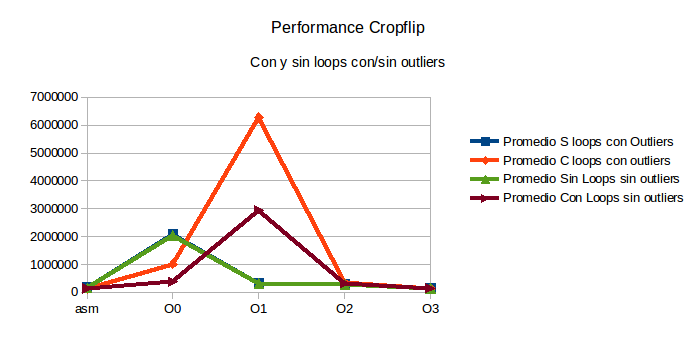
\includegraphics[scale=0.66]{Graficos1.4/1.3/per.png}
	\label{nombreparareferenciar1}
  \end{center}
\end{figure}
\\
Realizamos un cálculo de la varianza para ver qué tan precisos son los resultados y se obtiene esto:

\begin{figure}[h!]
  \begin{center}
	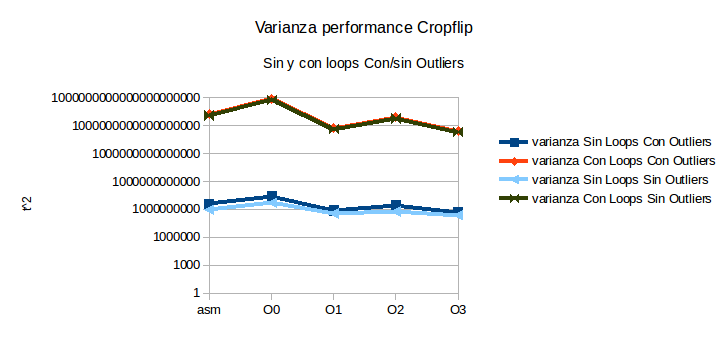
\includegraphics[scale=0.66]{Graficos1.4/1.3/var.png}
	\label{nombreparareferenciar2}
  \end{center}
\end{figure}

\newpage
\section{Cropflip}
\subsection{Diferencias de performance en Cropflip}
En el siguiente experimento se medirán las performances tanto de nuestro algoritmo en assembler, implementado para sacar provecho de las instrucciones SSE de Intel, como una versión alternativa hecha en C con diversos grados de optimización a cargo del compilador.

El algoritmo de Cropflip en assembler es muy sencillo. Simplemente movemos 128-bits de la imagen a un xmm y de allí al destino, que previamente ha sido seteado para colocar los bits en el lugar correcto. De esta manera, podremos mover de una sola vez, 16 bytes, lo que corresponde a 4 píxels de la imagen.

Dado que la cantidad de columnas es siempre múltiplo de 4, o sea, siempre tenemos 4 bytes para tomar, no es necesario chequear otros casos borde.

Las pruebas de performance, realizadas de la misma manera en que concluimos la anterior sección, se realizaron corriendo 4 loops en paralelo junto con los algoritmos de manera de minimizar el ruido y luego quitando los outliers.

Lo obtenido en los tests puede verse en el siguiente gráfico:

\begin{figure}[h!]
  \begin{center}
	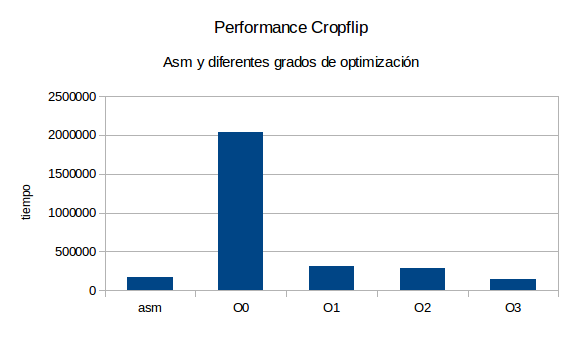
\includegraphics[scale=0.66]{Graficos1.4/crop/per.png}
	\label{nombreparareferenciar5}
  \end{center}
\end{figure}

\newpage
Y las varianzas son:

\begin{figure}[h!]
  \begin{center}
	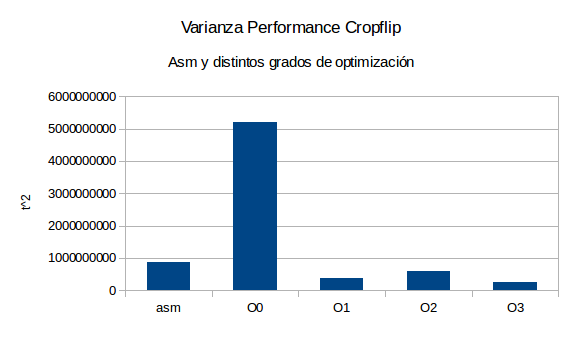
\includegraphics[scale=0.66]{Graficos1.4/crop/var.png}
	\label{nombreparareferenciar6}
  \end{center}
\end{figure}

De aquí puede verse que la implementación en assembler es tan buena como la implementación en C con el máximo grado de optimización.

\newpage

\subsection{cpu vs. bus de memoria en Cropflip}

Para este experimento lo que hicimos fue agregar instrucciones aritméticas y ver como esto influía en el tiempo de ejecución.

Tambien hicimos lo mismo pero con instucciones de lectura-escritura en memoria. 

Probamos agregando $4$, $8$ y $16$ instrucciones de cada una por separado y comparamos las performance entre sí y con la versión original.

Lo que obtuvimos fue lo siguiente:

\begin{figure}[h!]
  \begin{center}
  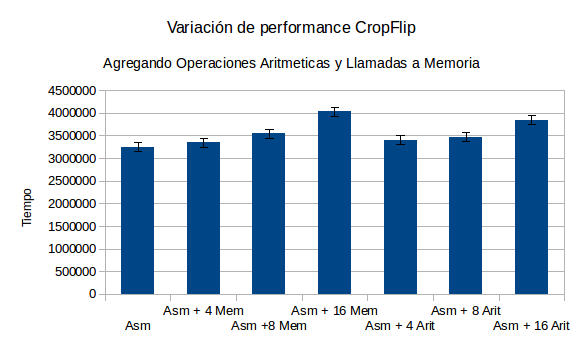
\includegraphics[scale=0.66]{Graficos1.5/crop/per.png}
  \label{nombreparareferenciar1}
  \end{center}
\end{figure}

\begin{figure}[h!]
  \begin{center}
  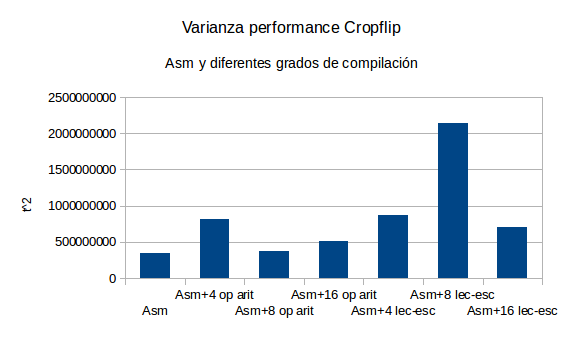
\includegraphics[scale=0.66]{Graficos1.5/crop/var.png}
  \label{nombreparareferenciar1}
  \end{center}
\end{figure}

==conculsión!!!==

\newpage
\section{Sierpinski}
\subsection{Diferencias de performance en Sierpinski}
Ahora analizamos el algoritmo del Sierpinski. En este caso, el algoritmo ya es un poco más complejo. Necesitamos calcular para cada píxel un coeficiente diferente, que dependerá de la posición (i,j) de cada píxel.
\\
Luego para poder paralelizar de alguna manera el algoritmo en C y sacar provecho a los registros xmm, es necesario calcular 4 coeficientes a la vez y multiplicárselos a sus respectivos píxels.
\\
Luego la idea del algoritmo será algo así:

\begin{itemize}
\item En la sección data guardamos una constante con el valor 255 brodcasteado en punto flotante.
\item Previo al ciclo, guardamos este valor en un registro.
\item Ya dentro del ciclo, leemos 4 píxels y los guardamos en un xmm.
\item A continuación calculamos de manera paralela para cada píxel el coeficiente correspondiente.
\item Primero, realizamos la división de i por la cantidad de filas y j por la cantidad de columnas, para la cual previamente pasamos de entero a punto flotante.
\item Multiplicamos ambos valores por 255 y luego convertimos a entero con truncamiento.
\item Realizamos un xor entre ambos y despues, volvemos a convertir a punto flotante para dividir por 255.
\item Ya con los coeficientes calculados, solo nos resta multiplicar cada uno por el píxel correspondiente.
\item Para ello desempaquetamos cada byte de cada píxel leido a word, y luego de word a dword, para así convertirlo a punto flotante.
\item Una vez hecha la conversión, brodcasteamos cada coeficiente para poder multiplicarlo por el píxel correspondiente.
\item Luego convertimos a entero nuevamente y empaquetamos todo de dword a word y de word a byte.
\item Y finalmente movemos los píxels procesados al destino.
\end{itemize}

Los resultados comparativos de performance para este algoritmo comparado con uno desarrollado en C fueron los siguientes:

\begin{figure}[h!]
  \begin{center}
  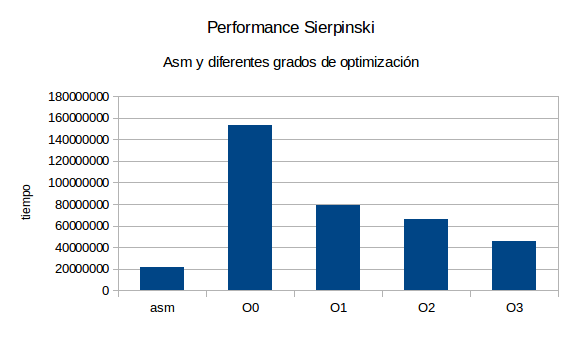
\includegraphics[scale=0.66]{Graficos1.4/sie/per.png}
  \label{nombreparareferenciar7}
  \end{center}
\end{figure}

\newpage

Y la varianza:

\begin{figure}[h!]
  \begin{center}
  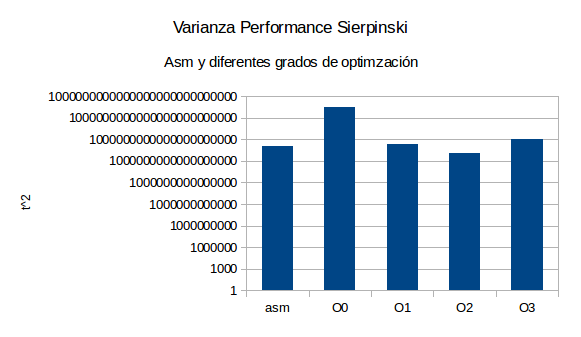
\includegraphics[scale=0.66]{Graficos1.4/sie/var.png}
  \label{nombreparareferenciar8}
  \end{center}
\end{figure}

Puede verse que en este caso nuestro modelo que toma y calcula de a 4 píxels utilizando instrucciones SIMD es incluso mejor que la versión de C con mayor grado de optimización.

\newpage
\subsection{cpu vs. bus de memoria en Sierpinski}

Realizamos el mismo experimento que hicimos para cropflip, es decir, agregando instrucciones aritmeticas y de lectura escritura y comparando las performances.

Graficando lo obtenido:

\begin{figure}[h!]
  \begin{center}
  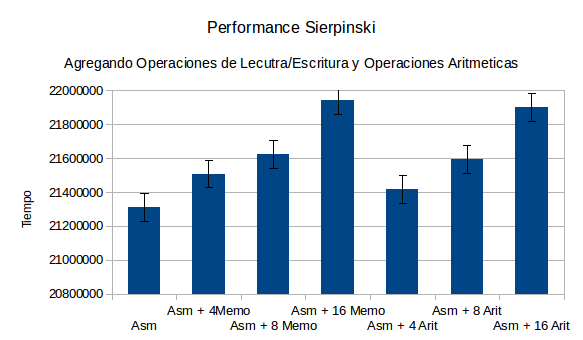
\includegraphics[scale=0.66]{Graficos1.5/sie/per.png}
  \label{nombreparareferenciar1}
  \end{center}
\end{figure}

\begin{figure}[h!]
  \begin{center}
  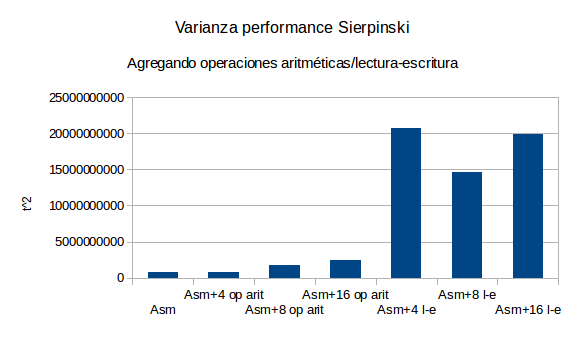
\includegraphics[scale=0.66]{Graficos1.5/sie/var.png}
  \label{nombreparareferenciar1}
  \end{center}
\end{figure}

==CONCLUSIÓN==

\newpage
\section{Bandas}
\subsection{Diferencias de performance en Bandas}
Para el algoritmo de bandas se nos presenta otro desafío: debemos tomar los tres colores de la imagen(r,g,b), sumarlos, y luego comparar cada uno de ellos para ver si se encuentra en un rango determinado.
\\
Para resolver la primera problemática usaremos las instrucciones $phaddw$, que nos permitirá a través de una suma horizontal, sumar los valores r,g,b de manera cómoda solamente utilizando dos registros.
\\
El segundo problema será comparar estos valores obtenidos en la suma de una manera eficiente. Querríamos compararlos todos a la vez y a partir de esas comparaciones determinar que valores deberá ir en cada píxel. Esta se resolverá utilizando broadcasting. El algoritmo irá comparando en cada paso contra un valor y en caso de cumplirse una condición, restará donde corresponda.


\begin{itemize}
\item  En la sección data tenemos mascaras y constantes brodcasteadas que utilizaremos para hacer las comparaciones.
\item  Ademas en esta sección tenemos una doble qword la cual usaremos para el shuffle final.
\item  Previo al ciclo donde procesamos los píxels, movemos estos datos a registros xmm.
\item  Ya una vez dentro del ciclo, leemos 4 píxels y los guardamos en un xmm.
\item  Desempaquetamos los bytes a word para poder hacer la suma de las componentes de cada píxel sin irnos de la representación.
\item  Hacemos dos sumas horizontales para obtener los cuatro valores  de b.
\item  Luego utilizamos las mascaras para comparar en paralelo cada píxel con el b correspondiente y asignando el valor de rgb segun corresponda.
\item  Nos queda en cada word de la parte baja de un xmm, los 4 valores que se asignaran a cada rgb de cada píxel.
\item  Finalmente, empaquetamos estos valores para volver a byte y los shuffleamos para dejarlos en los lugares correspondiente y lo asignamos en el destino.
\end{itemize}


Los resultados de los tiempos comparativos son los siguientes:

\begin{figure}[h!]
  \begin{center}
  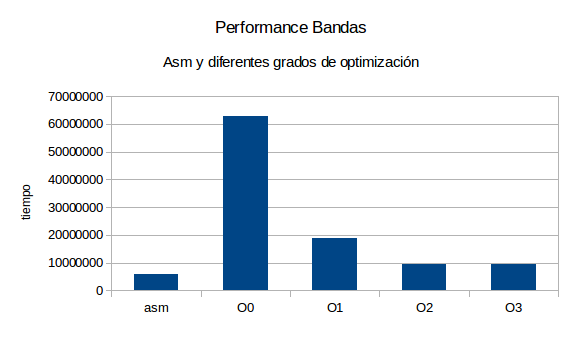
\includegraphics[scale=0.66]{Graficos1.4/ban/per.png}
  \label{nombreparareferenciar9}
  \end{center}
\end{figure}

\newpage
Y la varianza:

\begin{figure}[h!]
  \begin{center}
  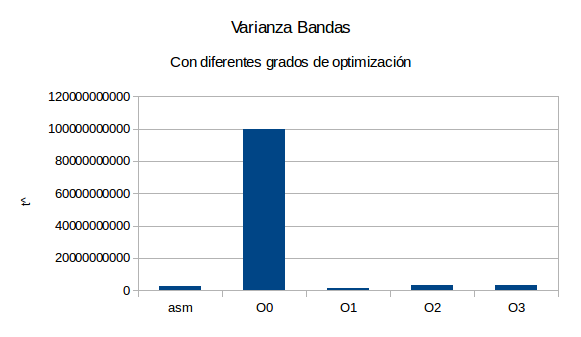
\includegraphics[scale=0.66]{Graficos1.4/ban/var.png}
  \label{nombreparareferenciar10}
  \end{center}
\end{figure}

Nuestro algoritmo obtiene una performance mucho mayor a la del código sin optimizar, y una performance casi idéntica al del código C con el mayor grado de optimización.

\newpage
\subsection{saltos condicionales}

En este experimento veremos como afectan los saltos condicionales a la performance del codigo C compilado con -O1. Para ello lo que haremos es quitar los IFs del codigo dejando solo una banda, luego medir la performance y compararla con la version con saltos.

\begin{figure}[h!]
  \begin{center}
  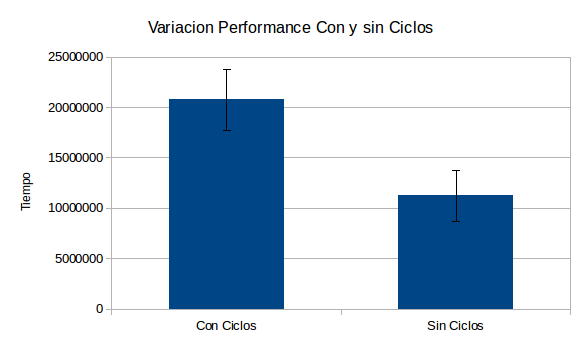
\includegraphics[scale=0.66]{Graficos3.1/per.png}
  \label{nombreparareferenciar1}
  \end{center}
\end{figure}

\begin{figure}[h!]
  \begin{center}
  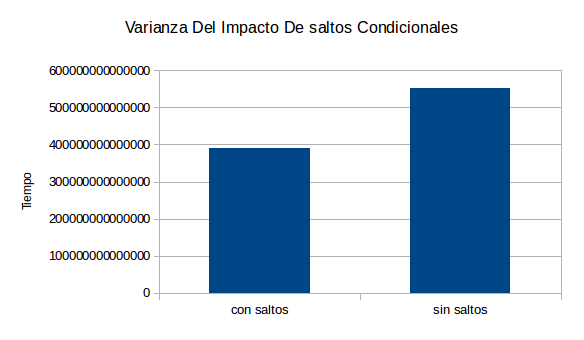
\includegraphics[scale=0.66]{Graficos3.1/var.png}
  \label{nombreparareferenciar1}
  \end{center}
\end{figure}

Como se puede ver en el gráfico del promedio, la versión de una sola banda tardó mucho menos con respecto a la versión original. Creemos que esta disminución en el tiempo de ejecución tiene que ver con la predicción de saltos del procesador. Esto se debe a que cuando hay un salto condicional, en principio el procesador no sabe a qué posición de memoria deberá dirigirse. Al haber removido estos saltos, tiene sentido que la performance se haya visto impactada de manera positiva. Con respecto a la varianza se ve que en la versión sin saltos es mucho menor respecto al original, es decir, los valores de la muestra se encuentran relativamente más cercanos al promedio.

\newpage
\subsection{Motion Blur}
\subsection{Diferencias de performance en Motion Blur}
Para este algoritmo por cada píxel se deben tomar 5 píxels, multiplicar cada uno de los colores por $0.2$ y luego sumarlos.
\\
Para ello debemos tener cuidado de tomar correctamente los casos borde y no aplicar motion blur donde no corresponde.
\\
Una idea general de cómo funciona el algoritmo en assembler es la siguiente:

\begin{itemize}
\item  Tenemos, en la sección datos, el valor $0.2$ brodcasteado que utilizaremos para realizar la multiplicación.
\item  Previo al procesamiento de datos, guardamos en un xmm este valor.
\item  Dentro del ciclo, para procesar el píxel (i,j) tomamos los 4 píxels de las filas $i-2$, $i-1$, $i$, $i+1$ e $i+2$ a partir de la columna $j-2$, $j-1$, $j$, $j+1$ y $j+2$, respectivamente, y almacenamos todo en registros.
\item  Desempaquetamos todo a word para poder hacer la suma sin desbordar.
\item  Luego de realizar las sumas, desempaquetamos a dwords para así poder convertir a punto flotante.
\item  Con la conversión ya hecha, podemos multiplicar cada valor por $0.2$.
\item  Convertimos a entero nuevamente y empaquetamos de dword a word y de word a byte.
\item  Finalmente, copiamos los 4 píxels resultantes al destino. 
\item  Cada vez que termino de recorrer una fila, pongo en negro los siguientes 4 píxels, y las dos primeras y últimas filas las pongo en negro aparte, fuera del ciclo.
\end{itemize}

Al realizar el testing se obtuvieron los siguientes resultados:

\begin{figure}[h!]
  \begin{center}
  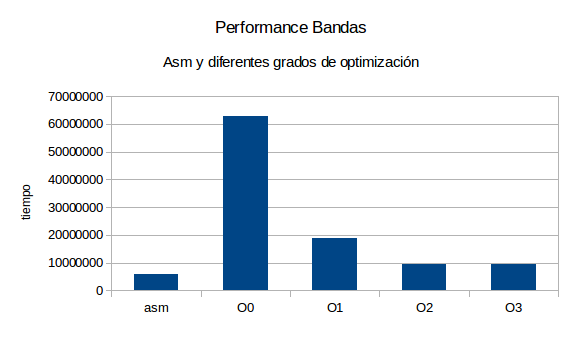
\includegraphics[scale=0.66]{Graficos1.4/ban/per.png}
  \label{nombreparareferenciar11}
  \end{center}
\end{figure}

Y la varianza:

\begin{figure}[h!]
  \begin{center}
  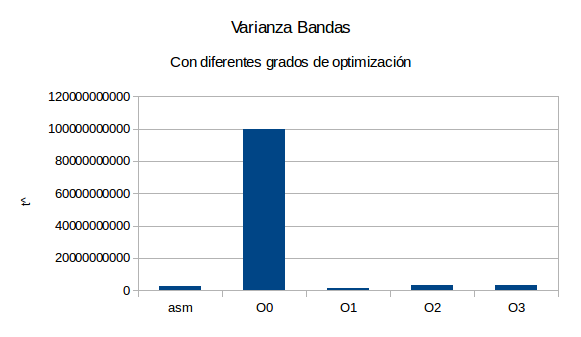
\includegraphics[scale=0.66]{Graficos1.4/ban/var.png}
  \label{nombreparareferenciar12}
  \end{center}
\end{figure}

En este caso nuestro algoritmo supera ampliamente incluso al código C con mayor grado de optimización.


\section{Conclusiones y trabajo futuro}



\end{document}

